
\documentclass[tikz,border=1pt]{standalone}
\usepackage{pgfplots,lmodern}
\pgfplotsset{compat=newest}

\definecolor{cfalconh1tiny90m}{HTML}{d9c2ff}
\definecolor{cfalconh105b}{HTML}{a665fe}
\definecolor{cfalconh1tinyr06b}{HTML}{994efe}
\definecolor{cfalconh115b}{HTML}{3e0a8a}
\definecolor{cfalconh115bdeep}{HTML}{3e0a8a}
\definecolor{cqwen2505b}{HTML}{c8d2ff}
\definecolor{cqwen2515b}{HTML}{1031da}
\definecolor{cgemma31b}{HTML}{0496fb}
\definecolor{cllama321b}{HTML}{b7d8ff}
\definecolor{cllama323b}{HTML}{04356f}
\definecolor{cphi35mini}{HTML}{aeb1b4}
\definecolor{cphi4mini}{HTML}{aeb1b4}
\definecolor{csmollm2360m}{HTML}{f8e599}
\definecolor{csmollm217b}{HTML}{f6d900}
\definecolor{ctinyllama11b}{HTML}{f0a855}
\definecolor{cinternlm2518b}{HTML}{23b953}

\begin{document}
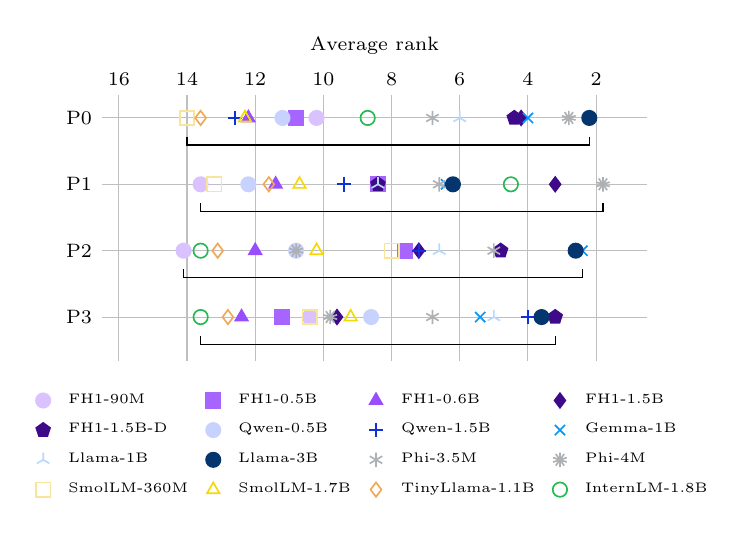
\begin{tikzpicture}[
  group line/.style={line width=0.45pt},
]

\begin{axis}[
  clip={false},
  grid={both},
  axis line style={draw=none},
  tick style={draw=none},
  tick label style={font=\scriptsize},
  label style={font=\scriptsize},
every axis plot/.append style={mark size=2.6pt, line width=0.4pt},
  xticklabel pos={upper},
  y dir={reverse},
  xmin={0.5},
  ymin={0.66},
legend style={
  draw=none,
  fill=none,
  at={(0.5,-0.08)},
  anchor=north,
  font=\fontsize{5.0}{6.2}\selectfont,
  row sep=.18em,
  column sep=.45em,
  /tikz/every odd column/.append style={column sep=.45em}
},
legend columns=4,
  legend cell align={left},
  title style={font=\scriptsize,yshift=.25\baselineskip},
  width={3.35in},
  ytick={1,2,3,4},
  yticklabels={{P0},{P1},{P2},{P3}},
  xmax={16.5},
  ymax={4.66},
  height={1.95in},
  x dir={reverse},
  cycle list={{cfalconh1tiny90m,mark=*,semithick},{cfalconh105b,mark=square*,semithick},{cfalconh1tinyr06b,mark=triangle*,semithick},{cfalconh115b,mark=diamond*,semithick},{cfalconh115bdeep,mark=pentagon*,semithick},{cqwen2505b,mark=otimes*,semithick},{cqwen2515b,mark=+,semithick},{cgemma31b,mark=x,semithick},{cllama321b,mark=Mercedes star,semithick},{cllama323b,mark=oplus*,semithick},{cphi35mini,mark=asterisk,semithick},{cphi4mini,mark=10-pointed star,semithick},{csmollm2360m,mark=square,semithick},{csmollm217b,mark=triangle,semithick},{ctinyllama11b,mark=diamond,semithick},{cinternlm2518b,mark=o,semithick}},
  xlabel={Average rank},
  legend columns={4},
]

\addplot+[only marks] coordinates {
  (10.2, 1)
  (13.6, 2)
  (14.1, 3)
  (10.4, 4)
};
\addlegendentry{FH1-90M}
\addplot+[only marks] coordinates {
  (10.8, 1)
  (8.4, 2)
  (7.6, 3)
  (11.2, 4)
};
\addlegendentry{FH1-0.5B}
\addplot+[only marks] coordinates {
  (12.2, 1)
  (11.4, 2)
  (12.0, 3)
  (12.4, 4)
};
\addlegendentry{FH1-0.6B}
\addplot+[only marks] coordinates {
  (4.2, 1)
  (3.2, 2)
  (7.2, 3)
  (9.6, 4)
};
\addlegendentry{FH1-1.5B}
\addplot+[only marks] coordinates {
  (4.4, 1)
  (8.4, 2)
  (4.8, 3)
  (3.2, 4)
};
\addlegendentry{FH1-1.5B-D}
\addplot+[only marks] coordinates {
  (11.2, 1)
  (12.2, 2)
  (10.8, 3)
  (8.6, 4)
};
\addlegendentry{Qwen-0.5B}
\addplot+[only marks] coordinates {
  (12.6, 1)
  (9.4, 2)
  (7.2, 3)
  (4.0, 4)
};
\addlegendentry{Qwen-1.5B}
\addplot+[only marks] coordinates {
  (4.0, 1)
  (6.4, 2)
  (2.4, 3)
  (5.4, 4)
};
\addlegendentry{Gemma-1B}
\addplot+[only marks] coordinates {
  (6.0, 1)
  (8.4, 2)
  (6.6, 3)
  (5.0, 4)
};
\addlegendentry{Llama-1B}
\addplot+[only marks] coordinates {
  (2.2, 1)
  (6.2, 2)
  (2.6, 3)
  (3.6, 4)
};
\addlegendentry{Llama-3B}
\addplot+[only marks] coordinates {
  (6.8, 1)
  (6.6, 2)
  (5.0, 3)
  (6.8, 4)
};
\addlegendentry{Phi-3.5M}
\addplot+[only marks] coordinates {
  (2.8, 1)
  (1.8, 2)
  (10.8, 3)
  (9.8, 4)
};
\addlegendentry{Phi-4M}
\addplot+[only marks] coordinates {
  (14.0, 1)
  (13.2, 2)
  (8.0, 3)
  (10.4, 4)
};
\addlegendentry{SmolLM-360M}
\addplot+[only marks] coordinates {
  (12.3, 1)
  (10.7, 2)
  (10.2, 3)
  (9.2, 4)
};
\addlegendentry{SmolLM-1.7B}
\addplot+[only marks] coordinates {
  (13.6, 1)
  (11.6, 2)
  (13.1, 3)
  (12.8, 4)
};
\addlegendentry{TinyLlama-1.1B}
\addplot+[only marks] coordinates {
  (8.7, 1)
  (4.5, 2)
  (13.6, 3)
  (13.6, 4)
};
\addlegendentry{InternLM-1.8B}
\draw[group line] (axis cs:2.2,1.2832618025751072) -- ++(0pt,-3pt) -- ([yshift=-3pt]axis cs:14.0,1.2832618025751072) -- ++(0pt,3pt);
\draw[group line] (axis cs:1.8,2.2832618025751072) -- ++(0pt,-3pt) -- ([yshift=-3pt]axis cs:13.6,2.2832618025751072) -- ++(0pt,3pt);
\draw[group line] (axis cs:2.4,3.2832618025751072) -- ++(0pt,-3pt) -- ([yshift=-3pt]axis cs:14.1,3.2832618025751072) -- ++(0pt,3pt);
\draw[group line] (axis cs:3.2,4.283261802575107) -- ++(0pt,-3pt) -- ([yshift=-3pt]axis cs:13.6,4.283261802575107) -- ++(0pt,3pt);

\end{axis}
\end{tikzpicture}
\end{document}

